\chapter{Noncommutative Algebra}\label{chapter:nca}

    References for this chapter are~\citet{sontz_principal_2015-1,beggs_quantum_2020}.

\section{Coalgebras}\index{co-!algebra}

    Dual (in the categorical sense) to the definition of a (unital associative) algebra we have:
    \newdef{Coalgebra}{
        A vector space $C$ together with two linear maps $\Delta:C\rightarrow C\otimes C$ and $\varepsilon:C\rightarrow K$, called the \textbf{comultiplication} and \textbf{counit}, that satisfy the following two axioms:
        \begin{enumerate}
            \item $(\mathbbm{1}\otimes\Delta)\circ\Delta = (\Delta\otimes\mathbbm{1})\circ\Delta$, and
            \item $(\mathbbm{1}\otimes\varepsilon)\circ\Delta = (\varepsilon\otimes\mathbbm{1})\circ\Delta = \mathbbm{1}$.
        \end{enumerate}
    }
    \begin{example}
        The simplest example is given by the vector space $V$ with basis $\{e_i\}_{i\in I}$ where the comultiplication and counit are defined as follows:
        \begin{gather}
            \Delta(e_i) := e_i\otimes e_i
        \end{gather}
        and
        \begin{gather}
            \varepsilon(e_i) := 1\,.
        \end{gather}
        By linearity these maps can be extended to all of $V$. Important cases are the tensor algebra and exterior algebra over a vector space (\namecrefs{vector:tensor_algebra}~\ref{vector:tensor_algebra} and~\ref{vector:exterior_algebra}).
    \end{example}
    \remark{This example shows that every algebra admits a coalgebra structure. However, this does not mean that every algebra admits the structure of a bialgebra (see below).}

    \newdef{Grouplike element}{
        An element $c$ in a coalgebra $(C,\Delta,\varepsilon)$ that satisfies $\Delta(c) = c\otimes c$ and $\varepsilon(c) = 1$.
    }
    \sremark{The name `grouplike' stems from the fact that the coalgebra structure on the group algebra $K[G]$ is obtained by defining $\Delta(g) = g\otimes g$ for all $g\in G$.}

    \newdef{Unital coalgebra}{
        A coalgebra $(C,\Delta,\varepsilon)$ is said to be unital if it comes equipped with a coalgebra morphism $\eta:K\rightarrow C$. The element $\eta(1)$ is often also denoted by 1.
    }
    \newdef{Primitive element}{\index{primitive!element}
        An element $c$ in a unital coalgebra $(C,\Delta,\varepsilon)$ that satisfies $\Delta(c) = c\otimes1 + 1\otimes c$.
    }

    \newdef{Frobenius algebra}{\index{Frobenius!algebra}\label{nca:frobenius}
        A tuple $(A,\nabla,\eta,\Delta,\varepsilon)$ that satisfies the following conditions:
        \begin{enumerate}
            \item $(A,\nabla,\eta)$ is an associative algebra.
            \item $(A,\Delta,\varepsilon)$ is a coassociative coalgebra.
            \item The \textbf{Frobenius law} holds:
                \begin{gather}
                    (\mathbbm{1}_A\otimes\nabla)\circ(\Delta\otimes\mathbbm{1}_A) = \Delta\circ\nabla = (\nabla\otimes\mathbbm{1}_A)\circ(\mathbbm{1}_A\otimes\Delta)\,.
                \end{gather}
        \end{enumerate}
        If $\nabla\circ\Delta=\mathbbm{1}_A$, the algebra is said to be \textbf{special}.
    }
    \begin{remark}
        It is this definition that can be generalized to arbitrary symmetric monoidal categories.
    \end{remark}

    \begin{notation}[Sweedler notation]\index{Sweedler notation}\label{nca:sweedler_notation}
        Let $(C,\Delta)$ be a coalgebra. For any element $c\in C$ the comultiplication $\Delta(c)$ is an element of $C\otimes C$ and can thus be written in the following form \[\Delta(c) = \sum_{i\in I}a_i\otimes b_i\] for some finite index set $I$. For lengthy calculations with a lot of different symbols this notation gets tedious and, hence, the following shorthand\footnote{Sometimes the notation $\Delta(c) = \Delta_1(c)\otimes\Delta_2(c)$ is used.} is introduced:
        \begin{gather}
            \Delta(c) = \sum_{(c)}c_{(1)}\otimes c_{(2)}
        \end{gather}
        or even
        \begin{gather}
            \Delta(c) = c_{(1)}\otimes c_{(2)}\,.
        \end{gather}
        As an example the coassociativity condition $(\Delta\otimes\mathbbm{1})\circ\Delta = (\mathbbm{1}\otimes\Delta)\circ\Delta$ is rewritten: \[c_{(1)}\otimes c_{(2)}\otimes c_{(3)} = \sum_{(c)} c_{(1)(1)}\otimes c_{(1)(2)}\otimes c_{(2)} = \sum_{(c)} c_{(1)}\otimes c_{(2)(1)}\otimes c_{(2)(2)}\,.\] Analogously, the counit law becomes \[c = c_{(1)}\varepsilon(c_{(2)}) = \varepsilon(c_{(1)})c_{(2)}\] and, hence, one can freely move the counit $\varepsilon$ around.
    \end{notation}

    By dualizing the definition of ideals in a ring one obtains the following notion.
    \newdef{Coideal}{\index{co-!ideal}
        Let $(C,\Delta,\varepsilon)$ be a coalgebra. A subcoalgebra $I$ of $C$ is a (left) coideal if
        \begin{gather}
            \Delta(I)\subseteq C\otimes I\,,
        \end{gather}
        i.e.~it is a comodule with respect to the comultiplication.
    }

\section{Hopf algebras}

    \newdef{Bialgebra}{\index{bi-!algebra}
        Let $A$ be a vector space over a field $K$. Suppose that the triple $(A,\nabla,\eta)$ defines a unital associative algebra and that the triple $(A,\Delta,\varepsilon)$ defines a counital coassociative coalgebra. The quintuple $(A,\nabla,\eta,\Delta,\varepsilon)$ defines a bialgebra if $\nabla$ and $\Delta$ satisfy the commutative diagrams in \cref{fig:bialgebra}. These diagrams state that $\nabla,\eta$ are coalgebra morphisms and $\Delta,\varepsilon$ are algebra morphisms.
    }

    \begin{figure}[ht!]
        \centering
        \begin{subfigure}[b]{0.9\textwidth}
            \centering
            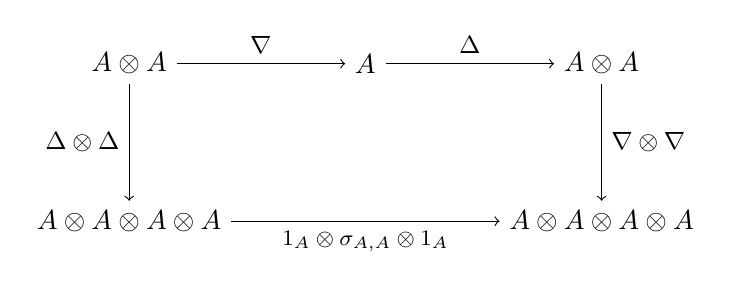
\begin{tikzpicture}
                \node (AA1) at (0, 0) {$A\otimes A$};
                \node (A) at (3, 0) {$A$};
                \node (AA2) at (6, 0) {$A\otimes A$};
                \node (AAAA1) at (0, -2) {$A\otimes A\otimes A\otimes A$};
                \node (AAAA2) at (6, -2) {$A\otimes A\otimes A\otimes A$};
                \draw[->] (AA1) -- node[above]{\small $\nabla$} (A);
                \draw[->] (A) -- node[above]{\small $\Delta$} (AA2);
                \draw[->] (AA1) -- node[left]{\small $\Delta\otimes\Delta$} (AAAA1);
                \draw[->] (AA2) -- node[right]{\small $\nabla\otimes\nabla$} (AAAA2);
                \draw[->] (AAAA1) -- node[below]{\footnotesize $\mathbbm{1}_A\otimes\sigma_{A,A}\otimes\mathbbm{1}_A$} (AAAA2);
            \end{tikzpicture}
        \end{subfigure}
        \par\bigskip
        \begin{subfigure}[b]{0.3\textwidth}
            \centering
            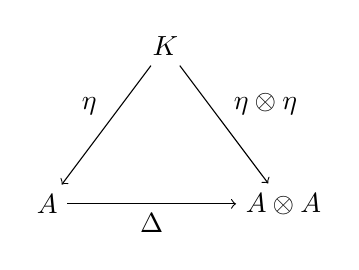
\begin{tikzpicture}
                \node (K) at (0, 0) {$K$};
                \node (A) at (-1.5, -2) {$A$};
                \node (AA) at (1.5, -2) {$A\otimes A$};
                \draw[->] (K) -- node[above left]{$\eta$} (A);
                \draw[->] (K) -- node[above right]{$\eta\otimes\eta$} (AA);
                \draw[->] (A) -- node[below]{$\Delta$} (AA);
            \end{tikzpicture}
        \end{subfigure}
        \begin{subfigure}[b]{0.3\textwidth}
            \centering
            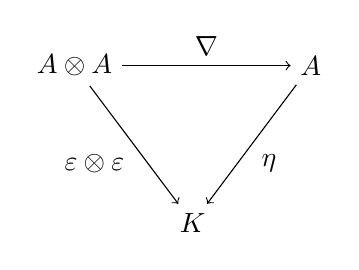
\begin{tikzpicture}
                \node (K) at (0, -2) {$K$};
                \node (AA) at (-1.5, 0) {$A\otimes A$};
                \node (A) at (1.5, 0) {$A$};
                \draw[<-] (K) -- node[below left]{$\varepsilon\otimes\varepsilon$} (AA);
                \draw[<-] (K) -- node[below right]{$\eta$} (A);
                \draw[->] (AA) -- node[above]{$\nabla$} (A);
            \end{tikzpicture}
        \end{subfigure}
        \begin{subfigure}[b]{0.3\textwidth}
            \centering
            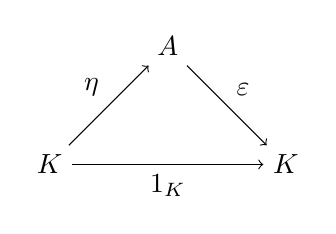
\begin{tikzpicture}
                \node (A) at (0, 0) {$A$};
                \node (K1) at (-1.5, -1.5) {$K$};
                \node (K2) at (1.5, -1.5) {$K$};
                \draw[->] (K1) -- node[above left]{$\eta$} (A);
                \draw[->] (A) -- node[above right]{$\varepsilon$} (K2);
                \draw[->] (K1) -- node[below]{$\mathbbm{1}_K$} (K2);
            \end{tikzpicture}
        \end{subfigure}
        \caption{Bialgebra conditions.}
        \label{fig:bialgebra}
    \end{figure}

    \newdef{Convolution}{\index{convolution}\label{nca:convolution}
        Let $(A,\nabla,\eta,\Delta,\varepsilon)$ be a bialgebra. The convolution of two morphisms $f,g:A\rightarrow A$ is defined as follows:
        \begin{gather}
            f\ast g := \nabla\circ(f\otimes g)\circ\Delta\,.
        \end{gather}
        When equipped with the convolution as multiplication, the space of morphisms on a bialgebra also becomes an algebra. In fact, this extends to morphisms between two algebras, turning $\mathbf{Alg}(A,A')$ into a $K$-algebra itself.
    }

    \newdef{Hopf algebra}{\index{Hopf!algebra}\index{antipode}\label{nca:hopf_algebra}
        A bialgebra $(A,\nabla,\eta,\Delta,\varepsilon)$ equipped with a linear map $S:A\rightarrow A$ that satisfies
        \begin{gather}
            \label{nca:hopf_algebra_relation}
            \nabla\circ(\mathbbm{1}_A\otimes S)\circ\Delta = \nabla\circ(S\otimes\mathbbm{1}_A)\circ\Delta = \eta\circ\varepsilon
        \end{gather}
        or, using the convolution on $A$,
        \begin{gather}
            \mathbbm{1}_A\ast S = S\ast\mathbbm{1}_A = \eta\circ\varepsilon\,.
        \end{gather}
        The map $S$ is called the \textbf{antipode} or \textbf{coinverse}.
    }
    \remark{Some authors require the antipode to be invertible. (In finite dimensions this is always the case as noted below.)}

    \begin{property}
        Given a Hopf algebra structure on a bialgebra, the antipode $S$ is an antihomomorphism. Furthermore, by noting that it is the inverse of the identity under convolutions, one can show that the antipode is unique (if it exists). Being a Hopf algebra is thus a property, not a structure.
    \end{property}
    \begin{example}[Finite-dimensional bialgebras]
        Any finite-dimensional bialgebra admits an invertible antipode and, in particular, is a Hopf algebra.
    \end{example}

    \begin{property}\label{nca:hopf_algebra_morphisms}
        The algebra $\mathbf{Alg}(H,H')$ of algebra morphisms between two Hopf algebras is a group under the convolution product in \cref{nca:convolution}. The inverse of a morphism $\phi$ is given by $\phi\circ S_H=S_{H'}\circ\phi$.
    \end{property}

    \newdef{Quasitriangular Hopf algebra\footnotemark}{\index{R-matrix}\index{quasi-!cocommutative}
        \footnotetext{Sometimes called a \textbf{braided Hopf algebra}.}
        A Hopf algebra $H$ for which there exists an invertible element $R\in H\otimes H$ that satisfies:
        \begin{enumerate}
            \item $R\Delta(a) = \sigma\bigl(\Delta(x)\bigr)R$,
            \item $(\Delta\otimes\mathbbm{1})(R) = R_{13}R_{23}$, and
            \item $(\mathbbm{1}\otimes\Delta)(R) = R_{13}R_{12}$,
        \end{enumerate}
        where $\sigma(x\otimes y) = y\otimes x$ is the braiding on $H$ and where $R_{ij}\in H\otimes H\otimes H$ is defined using the components of $R$ in the $i^{th}$ and $j^{th}$ position and the unit element $1\in H$ in the other position, i.e.~$(a\otimes b)_{13} = a\otimes1\otimes b$.

        The element $R$ is often called the \textbf{universal $R$-matrix}\footnote{This name is in general used for all elements $R\in H\otimes H$ satisfying the first condition above.}. Any Hopf algebra admitting such an element is said to be \textbf{quasicocommutative}.
    }

    \begin{example}[Universal enveloping algebra]
        Let $\mathfrak{g}$ be a Lie algebra and consider its universal enveloping algebra $U(\mathfrak{g})$ from \cref{section:universal_enveloping_algebra}. This algebra admits a Hopf algebra structure with the following operations:
        \begin{align}
            \Delta(e_i) &:= e_i\otimes1+1\otimes e_i\,,\\
            \varepsilon(e_i) &:= 0\,,\\
            S(e_i) &:= -e_i\,.
        \end{align}
        It becomes quasitriangular when equipped with the trivial $R$-matrix $\mathbbm{1}_{\mathfrak{g}}\otimes\mathbbm{1}_{\mathfrak{g}}$.
    \end{example}

    \begin{remark}[Tensor product of modules]\index{Tannaka duality}
        One could ask where bialgebras and especially Hopf algebras naturally arise. Consider an algebra $A$ together with its category of modules $A\mathbf{Mod}$. Now one would like to define a monoidal structure on $A\mathbf{Mod}$ induced by the tensor product on $A$. However, this monoidal structure should be compatible with the action of $A$.

        The intuitive (left) action \[A\otimes(M\otimes_A N)\rightarrow M\otimes_AN: a\otimes m\otimes n\mapsto (am)\otimes n\] does not admit a suitable tensor unit due to its asymmetric definition. To obtain the correct definition, one could be inspired by group representations: $g\cdot(m\otimes n) = gm\otimes gn$. In this case one has the diagonal map $\Delta:G\rightarrow G\times G$ that can be used to act on both sides of the tensor product. One could then ask ``Why not just define the action of an algebra in the same way?'', i.e.~\[a\otimes (m\otimes n)\mapsto (am)\otimes(an)\,.\] However, because the action is required to be linear (after all it should be compatible with the algebra morphisms), this definition is not valid. To resolve this issue, the existence of an additional algebra morphism $A\rightarrow A\otimes A$ is required with which one can construct a suitable action as follows:
        \begin{gather}
            A\otimes(M\otimes_AN)\rightarrow M\otimes_AN:a\otimes m\otimes n\mapsto (a_{(1)}m)\otimes(a_{(2)}n)\,.
        \end{gather}
        Together with the usual conditions of an algebra action, one obtains exactly the requirement that $A$ should be a bialgebra. So if $A$ is a bialgebra, then $A\mathbf{Mod}$ will be a monoidal category (this is in fact an equivalence known as \textbf{Tannaka duality}).

        Now, one could require some more structure on $A\mathbf{Mod}$, for example that it admits duals. Consider an $A$-module $V$ together with its dual $V^*\cong\hom(V,\mathbb{C})$. Given a linear map $S:A\rightarrow A$ one could define a general action as follows:
        \begin{gather}
            (af)(v) := f\bigl(S(a)v\bigr)\,.
        \end{gather}
        The requirement that this is indeed an action leads to the requirement $S(ab)=S(b)S(a)$ on $S$, which is equivalent to requiring that $S$ is an algebra antihomomorphism. Together with the other compatibility conditions, such as that the evaluation and coevaluation maps induced by the underlying vector spaces are also $A$-module morphisms, one is led to the requirement that $A$ is a Hopf algebra. Hence, if $A$ is a Hopf algebra (with an invertible antipode), then $A\mathbf{Mod}$ will be a rigid monoidal category.

        One could even go further and require the representation category to be braided. This requirement then exactly leads to the Hopf algebra being quasitriangular (this also explains why these Hopf algebras are sometimes said to be braided).
    \end{remark}

\subsection{Drinfel'd double}

    One can easily generalize \cref{group:bicrossed_product} (when written in terms of group algebras) to the case of bialgebras by replacing the group comultiplication by a general comultiplication.
    \newdef{Bicrossed product of bialgebras}{\index{bicrossed product}
        Two bialgebras $A,B$ are said to form a \textbf{matched pair} (of bialgebras) if there exist actions $-\cdot-:A\otimes B\rightarrow B$ and $-^-:A\otimes B\rightarrow B$, compatible with the coalgebra structures, that satisfy the following equations:
        \begin{enumerate}
            \item $a\cdot(bc) = (a_{(1)}\cdot b_{(1)})(a_{(2)}^{b_{(2)}}\cdot c)$,
            \item $a\cdot1=\varepsilon(a)1$,
            \item $(ab)^c = a^{b_{(1)}\cdot c_{(1)}}b_{(2)}^{c_{(2)}}$,
            \item $1^b = \varepsilon(b)1$, and
            \item $a_{(1)}^{b_{(1)}}\otimes a_{(2)}\cdot b_{(2)} = a_{(2)}^{b_{(2)}}\otimes a_{(1)}\cdot b_{(1)}$.
        \end{enumerate}
        Given such a matched pair, one can define a Hopf algebra structure on $A\otimes B$ defined by the following operations:
        \begin{itemize}
            \item\textbf{Product}: $(a\otimes b)(c\otimes d) = a(b_{(1)}\cdot c_{(1)})\otimes b_{(2)}^{c_{(2)}}d$,
            \item\textbf{Coproduct}: $\Delta(a\otimes b) = (a_{(1)}\otimes b_{(1)})\otimes(a_{(2)}\otimes b_{(2)})$, and
            \item\textbf{Counit}: $\varepsilon(a\otimes b) = \varepsilon_A(a)\varepsilon_B(b)$.
        \end{itemize}
        If the bialgebras are equipped with antipodes, the bicrossed product admits an induced antipode:
        \begin{gather}
            S(a\otimes b) = S_B(b_{(2)})\cdot S_A(a_{(2)})\otimes S_B(b_{(1)})^{S_A(a_{(1)})}\,.
        \end{gather}
    }

    \begin{example}[Tensor product]
        In the case where the bialgebra actions are given by left multiplication with the counits, the bicrossed product is isomorphic to the tensor product.
    \end{example}

    \begin{construct}[Drinfel'd double\footnotemark]\index{Drinfel'd!quantum double}
        \footnotetext{Also known as the \textbf{quantum double} (especially in physics).}
        Consider a Hopf algebra $H$ (with invertible antipode). It can be shown that $H$ and $(H^{op})^*$ form a matched pair of bialgebras. The left and right actions are induced by pullback:
        \begin{align}
            (a\cdot f)(b) &= f\bigl(S^{-1}(a_{(2)})ba_{(1)}\bigr)\,,\\
            a^f &= f\bigl(S^{-1}(a_{(3)})a_{(1)}\bigr)a_{(2)}\,.
        \end{align}
        The resulting bicrossed product $(H^{op})^*\bowtie H$ is called the Drinfel'd double $D(H)$.
    \end{construct}
    \begin{example}[Drinfel'd double for groups]
        Consider a finite group $G$ together with its associated group algebra $\mathbb{C}[G]$. On this algebra one can put a Hopf algebra structure as follows:
        \begin{align}
            \Delta(g) &= g\otimes g\,,\\
            \varepsilon(g) &= 1\,.
        \end{align}
        On the other hand one can also put a Hopf algebra structure on the dual $\mathbb{C}[G]^*$:
        \begin{align}
            \Delta(P_g) &= \sum_{hh'=g}P_h\otimes P_{h'}\,,\\
            \varepsilon(P_g) &= \delta_{g,e}\,,
        \end{align}
        where the basis for $\mathbb{C}[G]^*$ is given by the `projections' $P_g:h\mapsto\delta_{g,h}$. Antipodes for both algebras are given by $S(g)=g^{-1}$ and $S(P_g)=P_{g^{-1}}$.

        @@ COMPLETE @@
    \end{example}

\section{Quantum groups}

    This section heavily builds upon the theory presented in \cref{chapter:lie}. The content is partially based on talks by \textit{Henriques}.

    \begin{construct}[Jimbo--Drinfeld]\index{Jimbo--Drinfeld}\index{Chevalley--Serre!relations}\index{deformation}\index{quantization|seealso{deformation}}
        Consider a Lie algebra $\mathfrak{g}$ together with its universal enveloping algebra $U(\mathfrak{g})$ constructed using the \textit{Chevalley--Serre relations} (see \cref{lie:enveloping_algebra_construct}):
        \begin{enumerate}
            \item $[H_i,H_j] = 0$,
            \item $[H_i,E_j] = a_{ij}E_j$,
            \item $[H_i,F_j] = -a_{ij}F_j$,
            \item $[E_i,F_j] = \delta_{ij}H_j$,
            \item $\text{ad}_{E_i}^{|a_{ij}|-1}(E_j) = 0$, and
            \item $\text{ad}_{F_i}^{|a_{ij}|-1}(F_j) = 0$.
        \end{enumerate}
         To obtain the quantum group $U_q(\mathfrak{g})$, which is also called a \textbf{deformation} or \textbf{quantization} of $U(\mathfrak{g})$, one replaces the generators $H_i$ by the following generators\footnote{To be complete one should also add generators $K_i^{-1}$ that act formally as inverses of the generators $K_i$.}:
        \begin{gather}
            K_i := q^{d_iH_i}\,,
        \end{gather}
        where $d_i := \frac{\langle\alpha_i,\alpha_i\rangle}{2}$ is related to the norm of the $i^{th}$ simple root. So, instead of the $H_i$ being functionals on the root lattice, one gets functions from the root lattice to the Laurent polynomials in $q$, i.e.~to $\mathbb{C}[q,q^{-1}]$.

        From this functional point of view one can rewrite the second and third relation as follows:
        \begin{align*}
            f\cdot E_i &= E_i\tau_{\alpha_i}(f)\,,\\
            f\cdot F_i &= F_i\tau_{-\alpha_i}(f)\,,
        \end{align*}
        where $f$ is a polynomial in the $H_i$'s and $\tau_{\alpha_i}(f)(\lambda) := f(\lambda+\alpha_i)$. Replacing $H_i$ by $K_i$ one obtains the following relations:
        \begin{enumerate}
            \item[$2^*.$] $K_iE_j = q^{d_ia_{ij}}E_jK_i$, and
            \item[$3^*.$] $K_iF_j = q^{-d_ia_{ij}}F_jK_i$.
        \end{enumerate}
        The three relations between the $E_i$'s and the $F_i$'s are deformed using $q$-analog numbers. First, define the $q$-numbers\footnote{Note that $q$-numbers are often defined differently. This definition is equal to $\frac{1}{q^{n-1}}[n]_{q^2}$ when rewritten using the common definition.}:
        \begin{gather}
            [n]_q := \frac{q^n - q^{-n}}{q - q^{-1}}\,.
        \end{gather}
        Using this definition Serre relation 4 becomes
        \begin{enumerate}
            \item[$4^*.$] $[E_i,F_j] = \delta_{ij}[H_i]_{q^{d_i}} = \delta_{ij}\frac{K_i - K_i^{-1}}{q^{d_i} - q^{-d_i}}$,
        \end{enumerate}
        where the factor $[H_i]_{q^{d_i}}$ should be interpreted as first evaluating $H_i$ on a root and then taking the $q$-analog. The adjoint action relations (5 and 6) on $E_i$ and $F_i$ can be rewritten by replacing binomial coefficients by their $q$-analogs ($i\neq j$):
        \begin{enumerate}
            \item[$5^*.$] $\sum_{k=1}^{1-a_{ij}} (-1)^k\begin{bmatrix}1-a_{ij}\\k\end{bmatrix}_{q^{d_i}}E_i^{1-a_{ij}-k}E_jE_i^k = 0$, and
            \item[$6^*.$] $\sum_{k=1}^{1-a_{ij}} (-1)^k\begin{bmatrix}1-a_{ij}\\k\end{bmatrix}_{q^{d_i}}F_i^{1-a_{ij}-k}F_jF_i^k = 0$.
        \end{enumerate}
    \end{construct}

\section{Differential structures}
\subsection{Differential calculi}

    \newdef{First-order differential calculus}{\index{differential}\index{calculus}\index{differentiable}\label{nca:fodc}
        Let $A$ be an associative algebra and let $\Gamma$ be an $A$-bimodule. Together with an $A$-bimodule morphism $\dr:A\rightarrow\Gamma$ this structure is called a first-order differential calculus (FODC) if it satisfies the following two conditions:
        \begin{enumerate}
            \item\textbf{Leibniz rule}: $\dr(ab) = (\dr a)b + a(\dr b)$.
            \item\textbf{Standard form}: Every element $g\in\Gamma$ can be written as \[g = \sum_{i=1}^na_i(\dr b_i)\]
            for some $n\in\mathbb{N}$ and (not necessarily unique) elements $\{a_i,b_i\}_{i\leq n}$.
        \end{enumerate}
        If $\ker(\dr)\cong K$, where $K$ is the underlying field, the calculus is said to be \textbf{connected}. A calculus is said to be \textbf{inner} if the differential $d$ acts through a commutator, i.e.~there exists an element $\theta\in A$ such that $\dr a=[\theta,a]$ for all $a\in A$.

        An algebra morphism $\phi:A\rightarrow B$ is said to be \textbf{differentiable}, with respect to a choice of FODCs on $A$ and $B$, if there exists an $A$-bimodule morphism $\phi_*:\Gamma_A\rightarrow\Gamma_B$ ($A$ inherits an action on $\Gamma_B$ through $\phi$) such that $\dr\circ\phi=\phi_*\circ\dr$. If such a morphism exists, it is given by $\phi_*(a\dr b)=\phi(a)\dr\phi(b)$.
    }
    \remark{The second condition can be rewritten in terms of a right action using the Leibniz rule.}

    \newdef{Cotangent dimension}{\index{dimension!cotangent}\index{parallelizable}
        If $\Gamma$ is free over $A$ with a basis of cardinality $n$, it is said to be \textbf{parallelized with cotangent dimension} $\dim(A)-1$.

        This is in analogy with the case of function algebras $C^\infty(M)$ and the first de Rham space $\Omega^1(M)$ on a smooth manifold. If $\Omega^1(M)$ is free over $C^\infty(M)$, this implies that there exists a global basis of one-forms or, equivalently, a global frame of the tangent bundle. This is the same as saying that $M$ is parallelizable. (The cotangent dimension will be explained later.)
    }

    \begin{example}[Universal FODC]
        Consider an algebra $A$ with multiplication $\mu$. The bimodule $\Omega_\text{uni}:=\ker(\mu)$, equipped with the operator $\dr a:=1\otimes a-a\otimes1$, defines a first-order differential calculus on $A$. Furthermore, every FODC over $A$ can be obtained as the quotient $\Omega_\text{uni}/\mathcal{N}$ for a subbimodule $\mathcal{N}$. The universal FODC is inner if and only if there exists a central element $F\in A\otimes A$ such that $\mu(F)=1$.
    \end{example}
    \begin{example}[K\"ahler differentials]\index{K\"ahler!differential}
        In commutative algebra one has an equivalent construction. There one takes the module $\Omega^1(A)$ to be the quotient $I/I^2$, where $I$ is the again the augmentation ideal $I:=\ker(\mu)$. The quotient enforces that the bimodule is symmetric and, hence, that the Leibniz rule becomes
        \begin{gather}
            \dr(ab) = a\dr b + b\dr a\,.
        \end{gather}
        The module of K\"ahler differentials plays the same role as the universal FODC in commutative algebra in that it is universal with respect to modules over commutative algebras equipped with a derivation.
    \end{example}

    \newdef{Differential calculus}{\index{calculus}\index{exterior!algebra}
        Consider an algebra $A$. A differential calculus over $A$ is an $A$-bimodule with the structure of differential graded algebra $(\Gamma^\bullet,\dr)$ such that $\Gamma^0=A$. If $\Gamma^\bullet$ is freely generated by $A$ and $\dr A$, then $(\Gamma^\bullet,\dr)$ is often called an \textbf{exterior algebra} over $A$.
    }

    \begin{property}[Prolongation]\label{nca:prolongation}
        Every FODC $(\Gamma,\dr)$ admits a maximal extension (or \textbf{prolongation}) to an exterior algebra. In degree $k$ it is obtained by taking
        \begin{gather}
            \Gamma^k := \underbrace{\Gamma\otimes_A\cdots\otimes_A\Gamma}_{k\text{ times}}\,,
        \end{gather}
        and modding out the ideal generated by the following relations:
        \begin{gather}
            \left\{\sum_ida_i\otimes\dr b_i+\dr u_i\otimes\dr v_i=0\,\middle\vert\,\sum_ia_i\dr b_i=\sum_i(\dr u_i)v_i\right\}\,.
        \end{gather}
        If one starts from the universal FODC over an algebra, the resulting differential calculus is again universal in the sense that all other differential calculi can be obtained by taking quotients by differential ideals.
    \end{property}

\subsection{Covariance}

    \newdef{Covariant FODC}{
        An FODC $(\Gamma,\dr)$ over a Hopf algebra $H$ is said to be left-covariant if it is a left $H$-comodule such that
        \begin{gather}
            \Phi(a\dr b) = \Delta(a)(\mathbbm{1}_H\otimes\dr)\Delta(b)\,.
        \end{gather}
    }